\chapter{Related Artificial Intelligence}

\subsection{The Reinforcement Learning Model}

\begin{figure}[bth]
  \center
  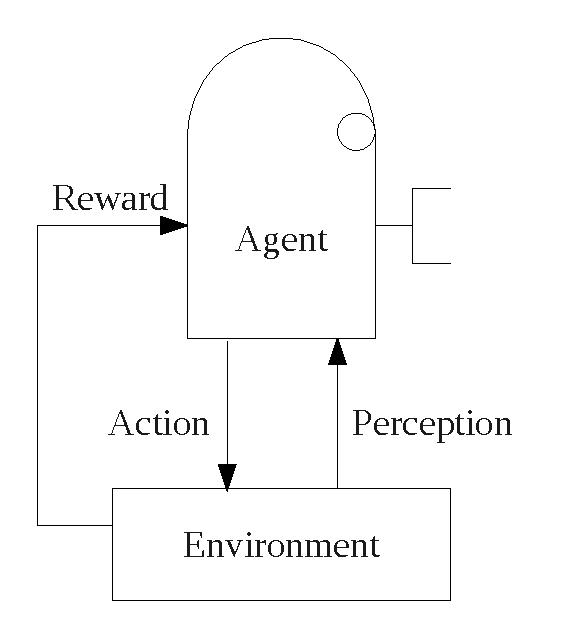
\includegraphics[height=5cm]{gfx/reinforcement_learning}
  \caption[The reinforcement learning model]{The reinforcement learning model.}
  \label{fig:reinforcement_learning}
\end{figure}

Figure~\ref{fig:reinforcement_learning} shows the basic reinforcement
learning model.  This model is an agent environment model, but there
is an extra information channel from the environment to the agent,
which communicates a numerical reward signal.  We can now say that the
agent has a learning problem.  The agent must learn what actions to
execute in order to gather the most reward.

\begin{figure}[bth]
  \center
  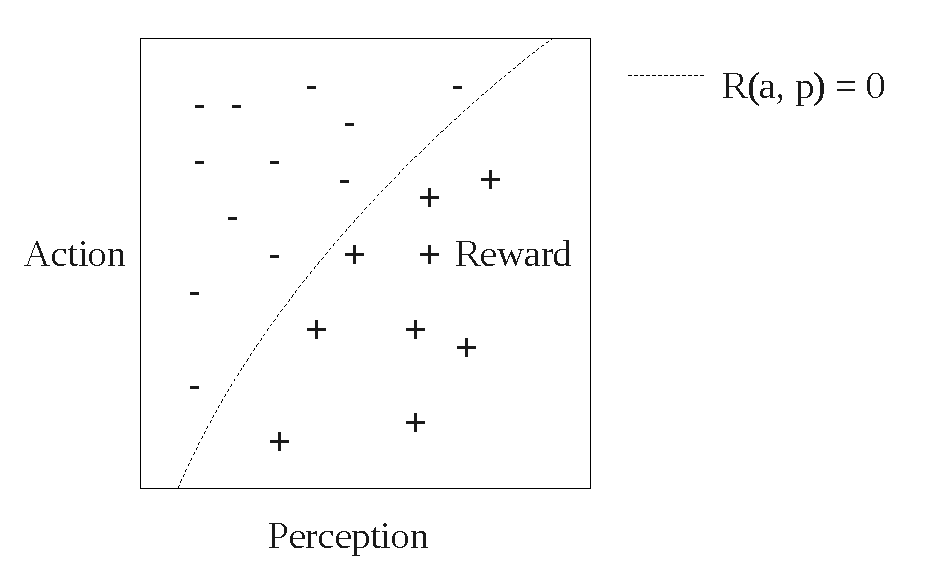
\includegraphics[height=4cm]{gfx/perception_categorization}
  \caption[Categorizing perceptions and actions based on goals]{Categorizing perceptions and actions based on goals.}
  \label{fig:perception_categorization}
\end{figure}

Once we have a basic reinforcement learning algorithm, we can approach
this learning problem as a function approximation problem.  In other
words, we can try to learn what parts of the perception and action
space have more or less reward.
Figure~\ref{fig:perception_categorization} shows a diagram of this
state space with the zero crossing of an approximation of the reward
plotted.

\subsection{Finding a Good Policy for Gathering Rewards}

Learning an approximation of what parts of a state space are good or
bad, based on reward, is not all that is needed to determine what
actions the agent should perform.  The agent wants to gather the most
rewards over time.  A simple way to formalize this problem is to learn
a policy that determines what action should be executed for every part
of the state space, based on some sort of summation of rewards over
time.  There have a been a number of ways of formalizing this
summation process as finite or infinite horizon problems
\citep{sutton:1998}.  Dynamic programming can be used for finding an
optimal or an approximately optimal policy \citep{bertsekas:1995}.

\subsection{Categorizing Perceptions and Actions based on Goals}

One problem with the reinforcement learning approach is that the only
representation of success or failure is a single number, the reward.
The basic reinforcement learning problem has been defined for finite
propositional state spaces.

A representation called \ac{RMDP} has been proposed
\citep{guestrin:2003} in order to extend reinforcement learning to
larger relational problem domains, but this method only focuses on an
object-oriented reward that does not have any global feedback about
the overall value of the situation.


